\documentclass[a4paper,10pt]{jsarticle}

% レイアウト
\setlength{\textwidth}{\fullwidth}
\setlength{\textheight}{39\baselineskip}
\addtolength{\textheight}{\topskip}
\setlength{\voffset}{-0.5in}
\setlength{\headsep}{0.3in}
\pagestyle{myheadings}

% パッケージ
\usepackage[dvipdfmx]{graphicx}
\usepackage{amsmath,amssymb,epsfig}
\usepackage{bm}
\usepackage{ascmac}
\usepackage{pifont}
\usepackage{multirow}
\usepackage{enumerate}
\usepackage{cases}
\usepackage{type1cm}
\usepackage{cancel}
\usepackage{url}
\usepackage{listings,jlisting}
% 大きな中括弧
\usepackage{cases}


% カウンタの設定
\setcounter{section}{0}
\setcounter{subsection}{0}
\setcounter{subsubsection}{0}
\setcounter{equation}{0}

% キャプションの図をFigに変更
\renewcommand{\figurename}{Fig.}
\renewcommand{\tablename}{Tab.}

% 式番号を式(章番号.番号)に
\makeatletter
\renewcommand{\theequation}{\arabic{section}.\arabic{equation}}
\@addtoreset{equation}{section}
\makeatother

% 表紙
\title{知能システム学特論レポート}
\author{
(DL2班)Caffe on Ubuntu\\
}
\date{2015年\ 6月\ 25日}

% ドキュメントの開始
\begin{document}
\maketitle
\section{報告者}
\begin{list}{}{}
 \item 15344203\hspace{0.5cm} 有田 裕太
 \item 15344206\hspace{0.5cm} 緒形 裕太
 \item 15344209\hspace{0.5cm} 株丹 亮
 \item 12104125\hspace{0.5cm} 宮本 和
\end{list}

\section{進行状況}
\begin{itemize}
\item 基本理論の研究
\item 第一層目の出力
\end{itemize}
\subsection{caffeの基本的なアルゴリズム}
\begin{lstlisting}[basicstyle=\ttfamily\footnotesize, frame=single, firstnumber=254, numbers=left]

\end{lstlisting}

\subsection{第一層目の出力}

\begin{lstlisting}[basicstyle=\ttfamily\footnotesize, frame=single]

\end{lstlisting}
%サンプル画像をFig.\ref{sample1}〜\ref{sample3}に示す. 


% \begin{figure}[t]
%  \begin{minipage}{0.33\hsize}
%   \begin{center}
%    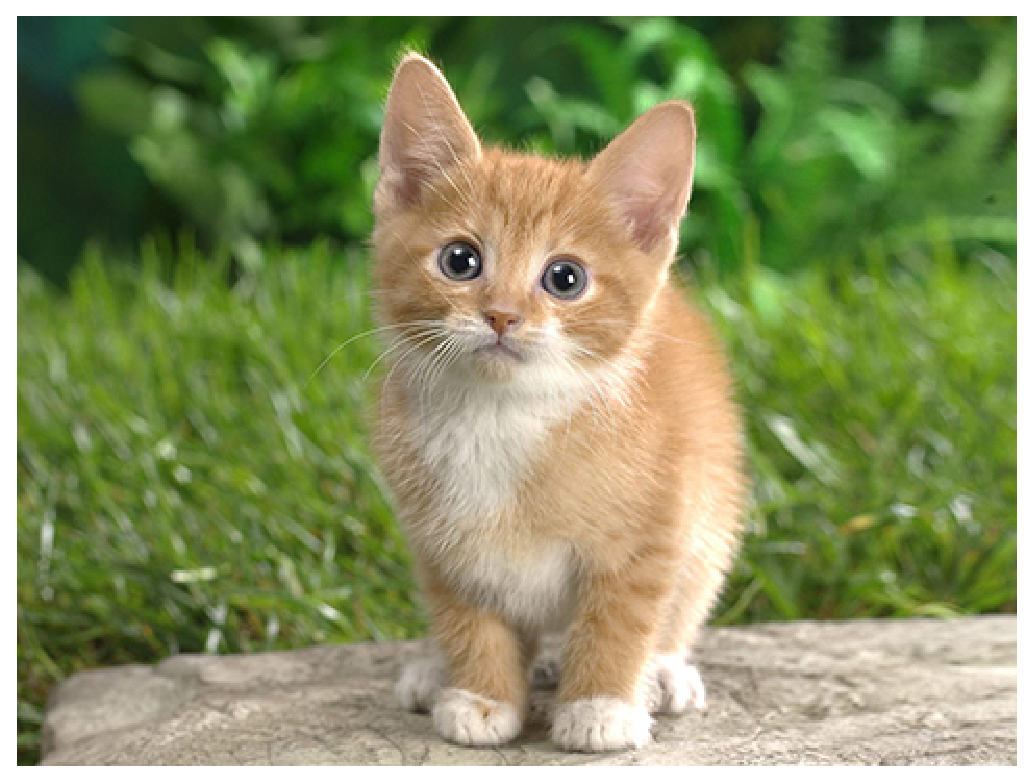
\includegraphics[width=50mm]{../02nd/fig/cat.eps}
%   \end{center}
%   \caption{sample1}
%   \label{sample1}
%  \end{minipage}
%  \begin{minipage}{0.33\hsize}
%  \begin{center}
%   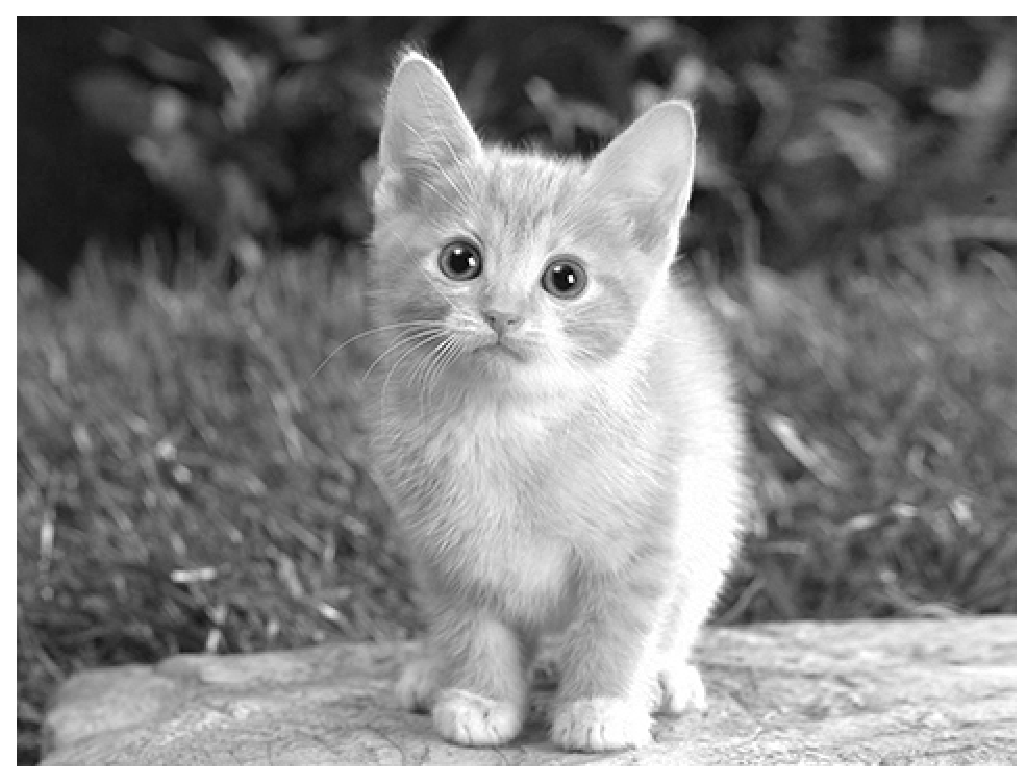
\includegraphics[width=50mm]{../02nd/fig/cat_gray.eps}
%  \end{center}
%   \caption{sample2}
%   \label{sample2}
%  \end{minipage}
%  \begin{minipage}{0.33\hsize}
%  \begin{center}
%   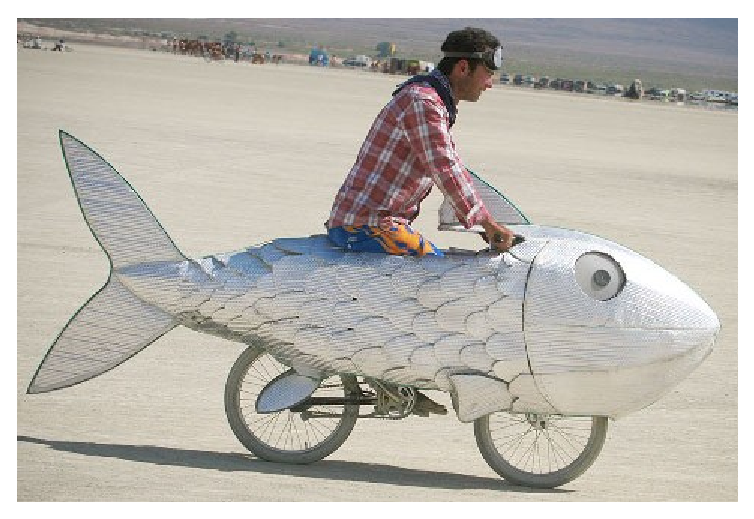
\includegraphics[width=50mm]{../02nd/fig/fish-bike.eps}
%  \end{center}
%   \caption{sample3}
%   \label{sample3}
%  \end{minipage}
% \end{figure}

% \begin{figure}[b]
%  \centering
%     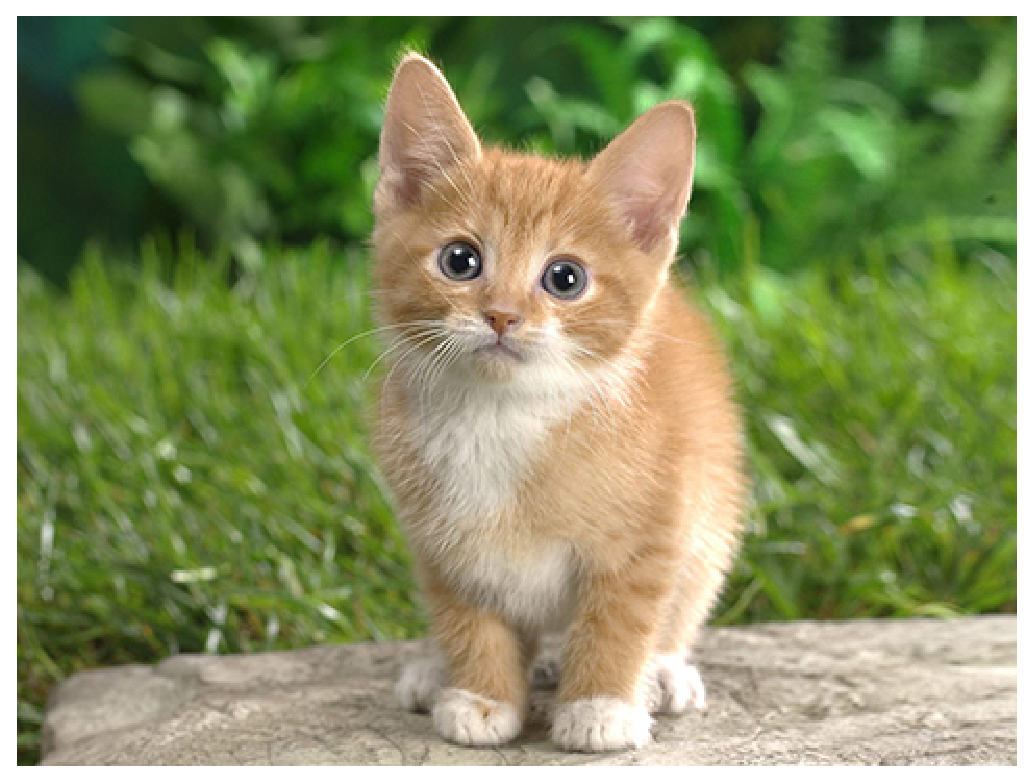
\includegraphics[width=50mm]{../02nd/fig/cat.eps}
%    \caption{sample1}
%    \label{sample1}
% \end{figure}
% \begin{figure}[b]
% \centering
%     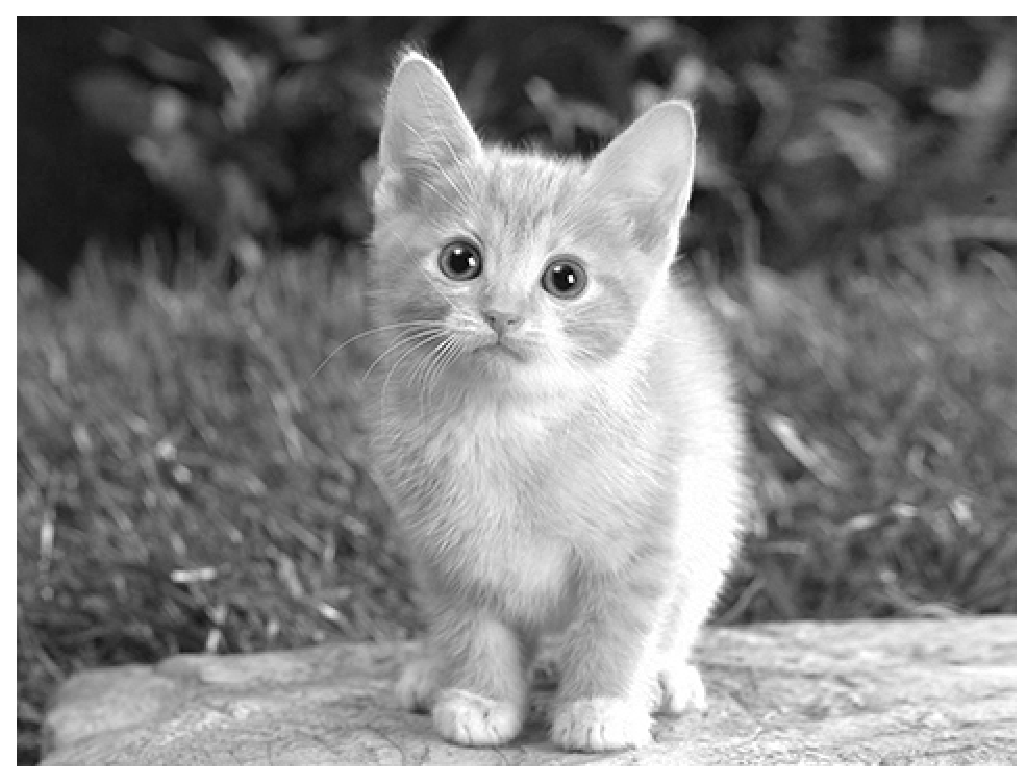
\includegraphics[width=50mm]{../02nd/fig/cat_gray.eps}
% \caption{sample2}
%  \label{sample2}
% \end{figure}
% \begin{figure}[b]
% \centering
%     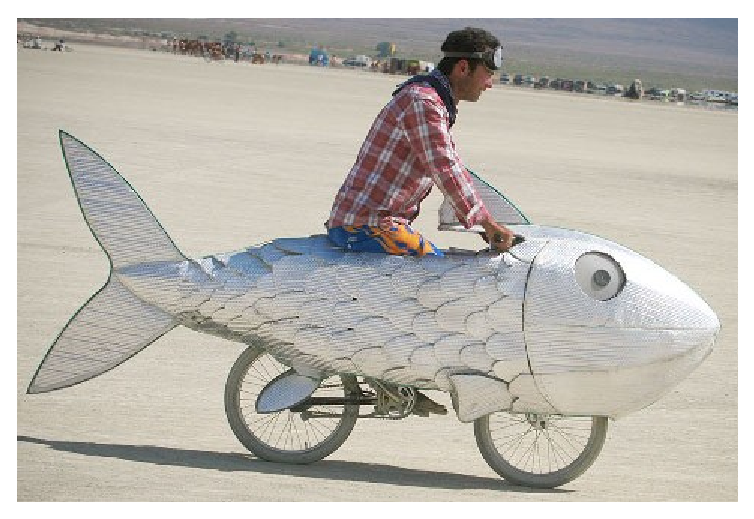
\includegraphics[width=50mm]{../02nd/fig/fish-bike.eps}
% \caption{sample3}
% \label{sample3}
% \end{figure}


\section{今後の課題}
\begin{itemize}
 \item 理論研究を進める.
 \item 中間層を更に出力,分析する.
\end{itemize}

\end{document}